\section{Introduction}
\textit{CausalTrail} is a tool for causal hypotheses testing.
It allows the formulation of three types of queries:
\begin{itemize}
 \item \texttt{Predictions},
 \item \texttt{Interventions},
 \item \texttt{Counterfactuals}.
\end{itemize}
\noindent
The graphical user interface is intended to simplify the usage of our tool.
This documentation introduces our graphical user interface and details how
it can be used.

\section{Build CausalTrail including the Graphical User Interface}
The following description is valid for linux systems only.
We use \textit{cmake} to build \textit{CausalTrail}.
There are two prerequisites that must be fulfilled to build our tool:
\begin{enumerate}
\item {The boost library, version 1.55.0 must be installed}
\item {A \textit{C++} compiler supporting \textit{C++11} must be installed}
\end{enumerate}
To build \textit{CausalTrail}, execute the following steps:
\begin{enumerate}
\item Go to the \textit{CausalTrail} directory
\item Create a \texttt{build} folder, e.g. by typing \texttt{mkdir build} in the console
\item Enter the \texttt{build} folder
\item Execute \textit{cmake} via \texttt{cmake ..}
\item Build the project by typing \texttt{make}
\item To build the tests of \textit{CausalTrail} enter the path to \textit{gtest} with the command \texttt{cmake . -DGTEST\_SRC\_DIR=<Path to gtest>}
\item Set the path to Qt by enter \texttt{cmake . -DQt5Widgets\_DIR=<Path to Qt>}
\item Build the project by typing \texttt{make}
\end{enumerate}
The executable of the gui is located in the folder \texttt{build/gui}, the consol version is located in the folder 
\texttt{build/core}, and tests can be found in the folder \texttt{build/test}.

\section{Supported Data Formats}
\subsection{Network Formats}
\textit{CausalTrail} supports the following network formats:
\begin{itemize}
 \item trivial graph format (tgf),
 \item simple interaction format (sif) and node attribute (na) files.
\end{itemize}

\subsubsection{Trivial Graph Format}
\label{subsection:tgf}
The \textit{Trivial Graph Format (TGF)} has the following structure:
\begin{center}
 \begin{tabular}{l}
	\texttt{NodeID	NodeAttribute}
	\\\texttt{...}
  	\\\texttt{\#}
    \\\texttt{NodeID	NodeID	EdgeAttribute}
	\\\texttt{...}
 \end{tabular}
\end{center}
The upper part of a \textit{TGF} file, contains the mapping between node identifiers and at most one optional attribute, e.g. node names. 
The \texttt{\#} marks the beginning of the actual network definition. Edges are directed from the first to the second node identifier.
An edge between two nodes can be mapped to at most one optional attribute.

\subsubsection{Node Attribute Format}
\label{subsection:na}
\textit{Node Attribute} files (NA) have the following structure:
\begin{center}
\begin{tabular}{l}
    \texttt{AttributeName (class	=	Type)}
    \\\texttt{NodeID	=	NodeAttribute}
    \\\texttt{...}
\end{tabular}
\end{center}
\noindent
Different node attribute classes can be referenced via the \texttt{AttributeName}. \texttt{Type} states the data type
of the node attributes in terms of a \textit{Java} class. The mapping of \texttt{NodeID} to \texttt{NodeAttribute} has to be unique within one class of attributes.

\subsubsection{Simple Interaction Format}
\label{subsection:sif}
The \textit{Simple Interaction Format (SIF)} has the following structure:
\begin{center}
\begin{tabular}{l}
 \texttt{...}
 \\\texttt{NodeID	EdgeType	NodeID}
 \\\texttt{...}
\end{tabular}
\end{center}
\noindent
Nodes in the network are identified via the \texttt{NodeID}. Therefore they have to be unique. 
The left \texttt{NodeID} represents the source of an edge, the right one represents the target. 
It is possible to assign more than one target node to a single source node, so multiple edges can be encoded in one line. 
The \texttt{Edge Type} encodes the type of an edge, e.g. whether an edge between two nodes is directed or not. It is also common to encode biological meaning in the \texttt{Edge Type}.
For example, \texttt{pd} represents Protein-DNA interactions, whereas \texttt{pp} represents Protein-Protein interactions. 
The \texttt{Edge Type} can also be longer string. This allows the encoding of more complex descriptions, e.g. \texttt{activates}, \texttt{inactivates}, or \texttt{phosphorylates}.
If it is not necessary to encode any specific meaning for an edge, \texttt{xx} or \texttt{yy} can be used as an \texttt{Edge Type}.

\subsection{Data}
\subsection{Discretisation Information}
\label{subsection:discInf}
The \textit{discretisation control file} is a regular text file.
Its rows are tab-delimited and structured as follows:
\begin{center}
\texttt{RowIndex	DiscretisationMethod	OptionalValue}
\end{center}
The \texttt{RowIndex} is the number of the row in the sample file upon which the specified discretisation method should 
be applied.
\\The \texttt{DiscretisationMethod} is an integer coding for one of the discretisation methods included in \textit{CausalTrail}.
The coding obeys the following system:
\begin{itemize}
	\item $0 \rightarrow$ Round to the next largest integer value.
	\item $1 \rightarrow$ Round to the next smallest integer value.
	\item $2 \rightarrow$ Round to the nearest integer value.
	\item $3 \rightarrow$ Thresholding according to the arithmetic mean.
	\item $4 \rightarrow$ Thresholding according to the harmonic mean.
	\item $5 \rightarrow$ Thresholding according to the  median.
	\item $6 \rightarrow$ Thresholding according to a manually set threshold.
	\item $7 \rightarrow$ Use the Bracket Median method.
	\item $8 \rightarrow$ Use the Pearson Tukey method.
	\item $9 \rightarrow$ The data is discrete.
	\item $10 \rightarrow$ Thresholding according to the Z-score.
\end{itemize}
The \texttt{OptionalValue} needs to be specified for methods $6$ and $7$.
Using our GUI, the \textit{discretisation control file} can be created interactively.                                                             

\mbox{}
\newpage
\section{Usage of the CausalTrail GUI}
Starting \textit{CausalTrail} causes the programme to search for a configuration file, containing the path to the data of the user.
If such a file could not be found, the user is asked to specify the path to the data. This is shown in Figure \ref{figure:causalTrailPath}.
\begin{figure}[H]
  \begin{center}
 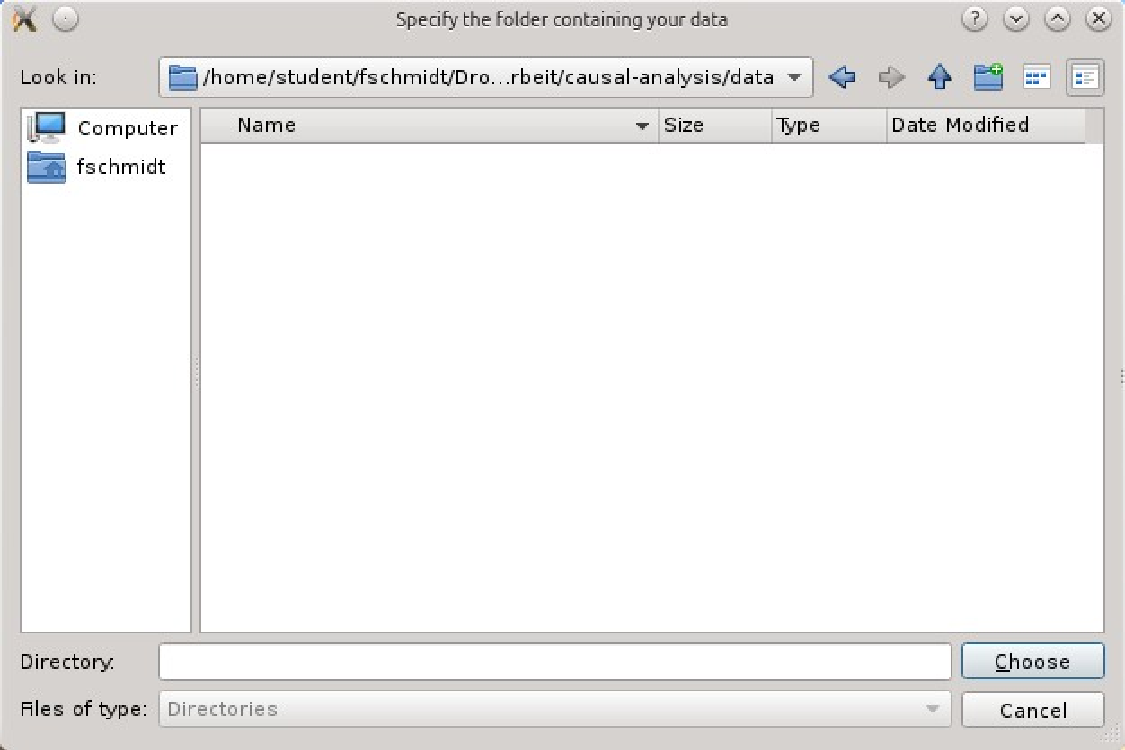
\includegraphics[width=6cm]{pic/path.eps}
 \end{center}
 \caption{Dialogue to specify the path to the data that should be used in \textit{CausalTrail}.}
 \label{figure:causalTrailPath}
\end{figure}
\noindent
The entered path is automatically saved into a configuration file for later usage.
\\The initial layout of \textit{CausalTrails} GUI is shown in Figure \ref{figure:causalTrailInitial}. At the bottom of the window,
there is a dock widget containing general information on the current session, labelled \texttt{Log}. At the top, there is a menu bar and
a toolbar allowing direct access to the most important actions.
At this stage, it is possible either to load a new network or to load a previously stored session. Loading networks is
covered in Section \ref{subsection:loadNetworks}, loading sessions is covered in Section \ref{subsection:loadSessions}.
\begin{figure}[H]
 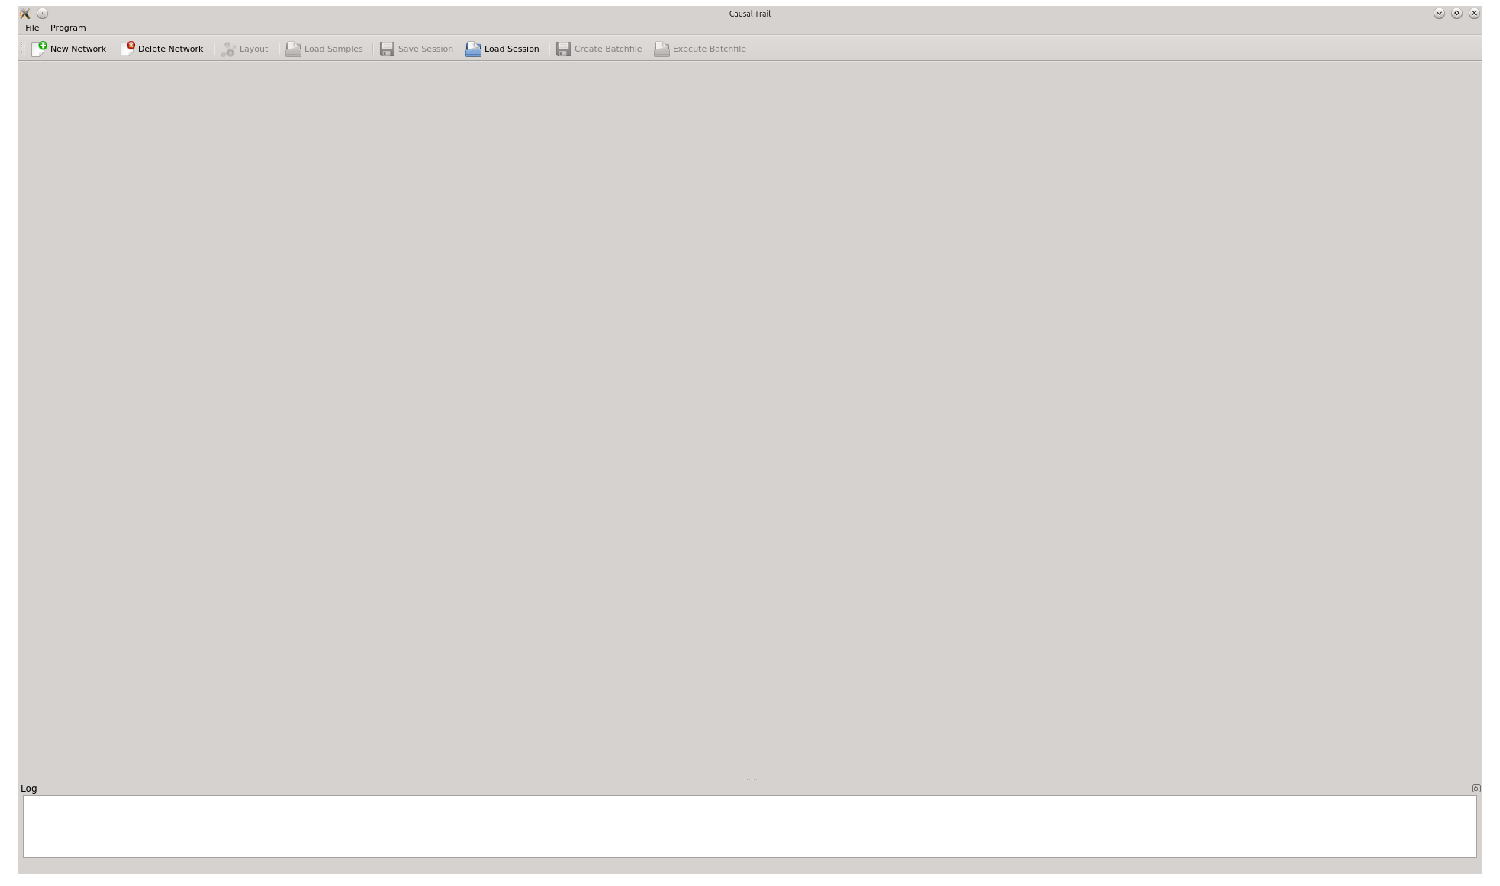
\includegraphics[width=\textwidth]{pic/gui1.eps}
 \caption{Initial layout of \textit{CausalTrail}. At this stage, the GUI consists of two main elements. The toolbar at the top and the \texttt{Log} widget at the bottom.
 The toolbar can be used to trigger all main actions that can be performed within \textit{CausalTrail}. The \texttt{Log} shows status reports for the current session of \textit{CausalTrail}.}
 \label{figure:causalTrailInitial}
\end{figure}

\subsection{Load a Network}
\label{subsection:loadNetworks}
Networks can be loaded by a click on \texttt{New Network} in the toolbar or by clicking on \texttt{File} $\rightarrow$ \texttt{New Network} in the menu.
Either actions open the dialogue shown in the left part of Figure \ref{figure:loadNetwork1}. The dialogue shows \textit{tgf} and \textit{na} files only. 
If a \textit{na} file is selected, another dialogue will pop up allowing to load the corresponding \textit{sif} file, as shown in the right part of Figure \ref{figure:loadNetwork1}.
\begin{figure}[H]
\begin{minipage}{6cm}
 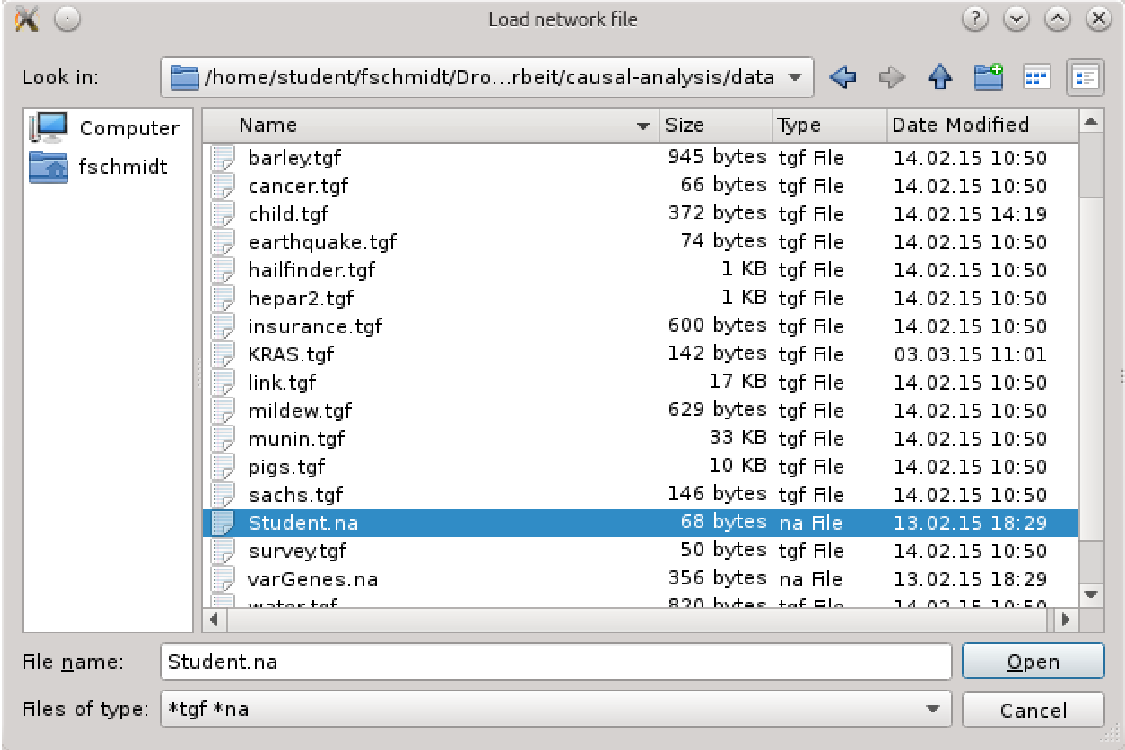
\includegraphics[width=6cm]{pic/network1.eps}
\end{minipage}
%
\begin{minipage}{6cm}
 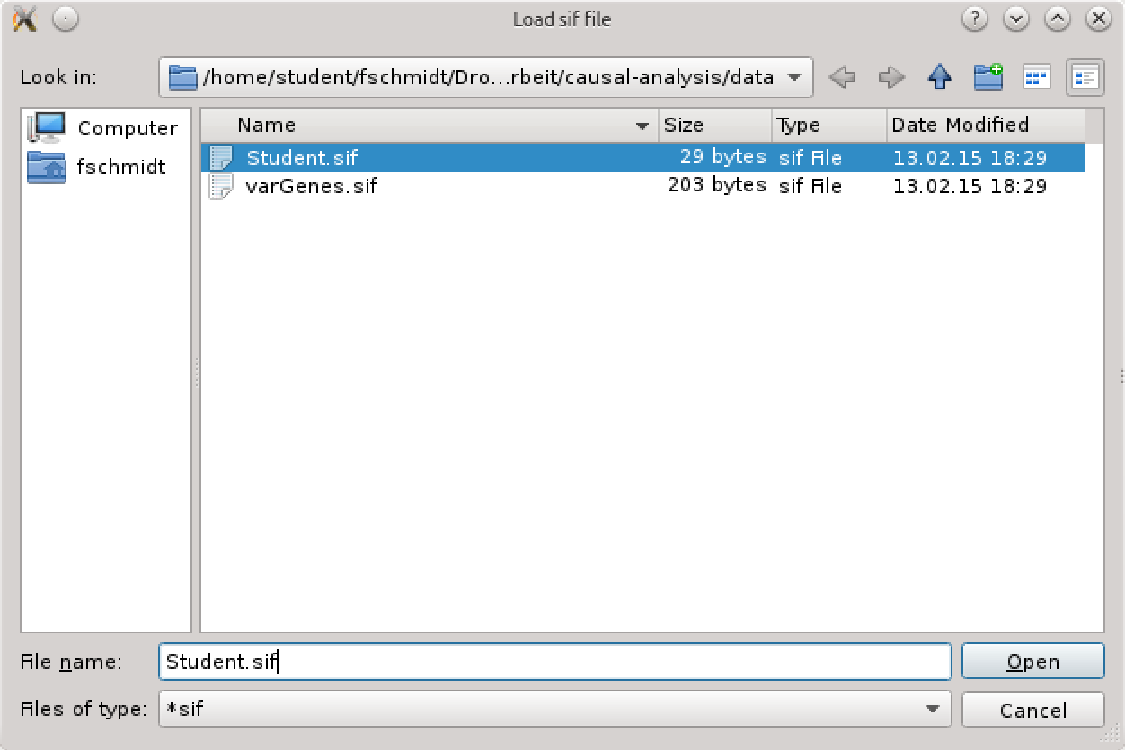
\includegraphics[width=6cm]{pic/network2.eps}
\end{minipage}
\caption{Dialogues to load networks. The dialogue on the left hand side can be used to load a \textit{tgf} or a \textit{na} file. The dialogue on the right hand-side is used to load a \textit{sif} file. It is shown if
a \textit{na} file was loaded beforehand.}
\label{figure:loadNetwork1}
\end{figure}

\noindent
\\Upon successfully reading the network it is visualised using a force directed graph layout. The network shown in Figure \ref{figure:networkExample} is the \textit{Student Network}
presented in \textit{Probabilistic Graphical Models} from \textit{Koller and Friedman}.  Nodes can be moved in the \texttt{Network Visualisation} widget. It is also possible to
zoom in our out of the view. The \texttt{Log} widget holds the path to the loaded files.
\begin{figure}[H]
 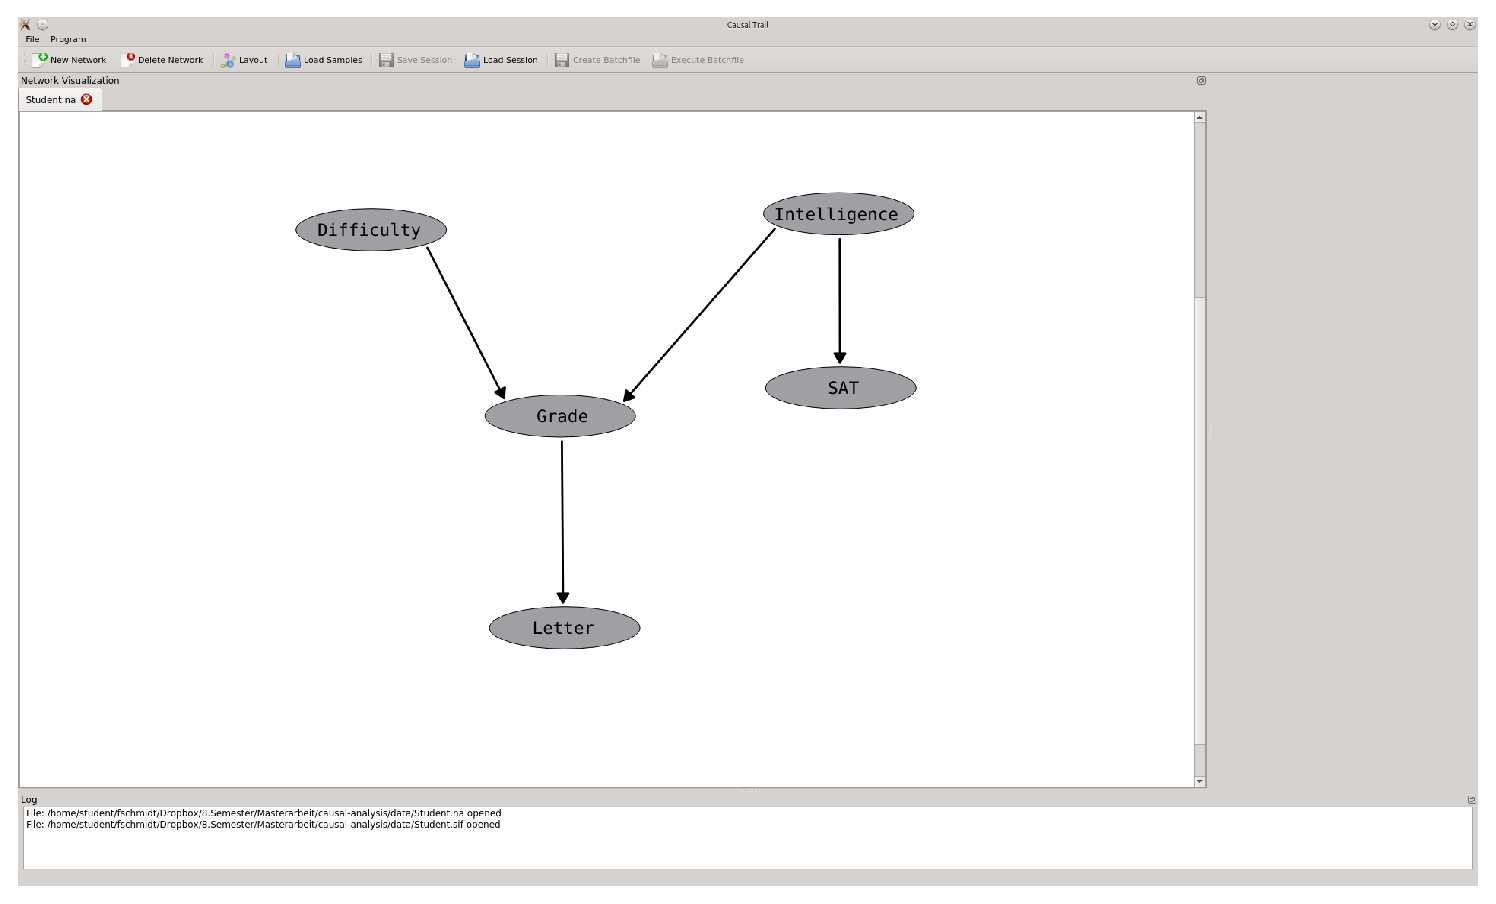
\includegraphics[width=\textwidth]{pic/gui2.eps}
 \caption{Visualisation of the \textit{Student Network} presented in \textit{Probabilistic Graphical Models} from \textit{Koller and Friedman}.}
 \label{figure:networkExample}
\end{figure}
\noindent
It is possible to layout the network again by clicking on \texttt{Layout} or by a click on \texttt{File} $\rightarrow$ \texttt{Layout}.
As soon as a network is loaded, it is possible to load samples. This is detailed in Section \ref{subsection:loadSamplesDiscretise}.
\bigskip
\\\textit{CausalTrail} allows the user to load multiple networks. Loading another network opens a new tab in the \texttt{Network Visualisation} widget. The user can switch between
loaded networks by clicking on the tabnames. The network that is currently visualised can be deleted by clicking on \texttt{Delete Network}. Alternatively, it can be deleted
by clicking on \texttt{File} $\rightarrow$ \texttt{Delete Network}.

\subsection{Load Samples and Discretise the Data}
\label{subsection:loadSamplesDiscretise}
To load samples, at least one network has to be loaded beforehand. Samples can be loaded by clicking 
on \texttt{Load Samples}, or by selecting \texttt{File} $\rightarrow$ \texttt{Load Samples} in the menu. 
Samples are loaded for the network shown in the \texttt{Network Visualisation} widget.
\\The aforementioned actions open the dialogue shown in Figure \ref{figure:loadData1}.
\begin{figure}[H]
\begin{center}
 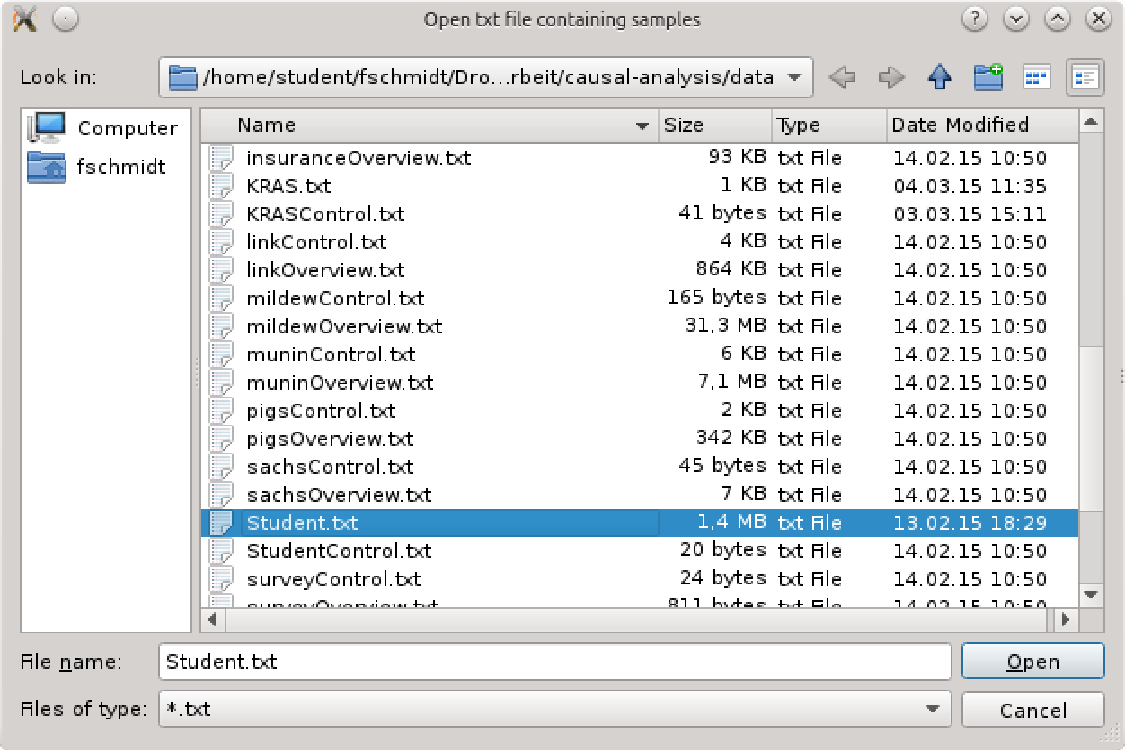
\includegraphics[width=8cm]{pic/loadData.eps}
 \caption{Dialogue to specify the name of the \textit{txt} file to be loaded.}
 \label{figure:loadData1}
\end{center}
\end{figure}
\noindent
Samples have to be encoded in  tab delimited \textit{txt} files. The first column of the sample file contains the names of the features, which have be equivalent to the node names in the selected network.
If there is no data provided for at least one node, the network can not be trained. The sample file must not contain column names. 
Upon selection of a file containing samples, the user is asked whether he wants to view the data or not. This is shown in Figure \ref{figure:loadData2}. Note that depending on the size of the dataset,
it might take a few seconds till the window containing the data appears.
\begin{figure}[H]
 \begin{center}
 
\includegraphics[width=4cm]{pic/dialogViewData.eps}
 \caption{The user can either view the actual data or proceed directly to the discretisation step.}
 \label{figure:loadData2}
 \end{center}
\end{figure}
\noindent
Visualising the data opens a new window, containing a table listing the samples of the specified file. As depicted in Figure \ref{figure:loadData3}, it is possible to exclude distinct samples from further usage.
\begin{figure}[H]
 \begin{center}
 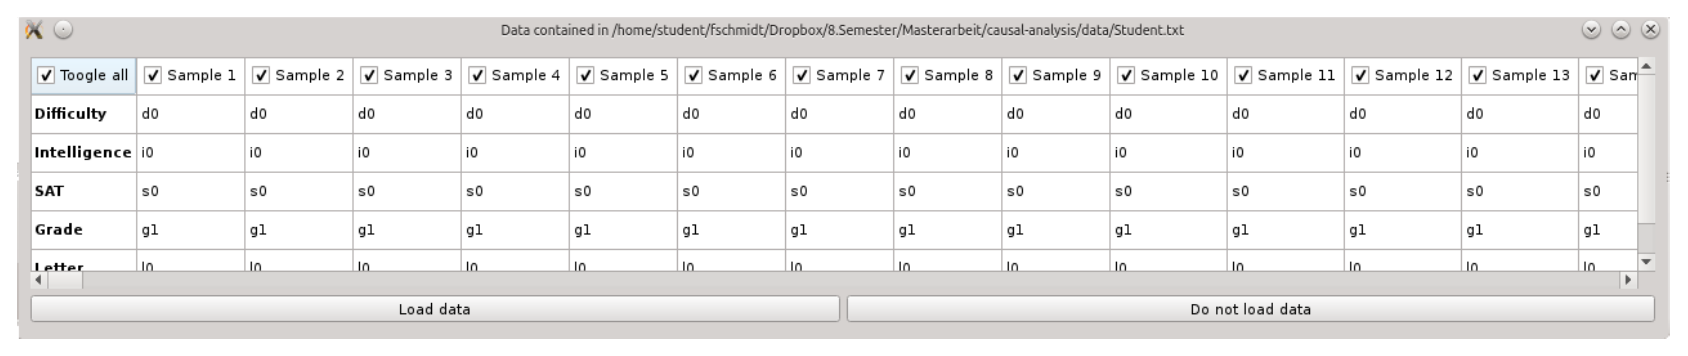
\includegraphics[width=\textwidth]{pic/dataView.eps}
 \caption{Visualisation of the Student data. Clicking on check boxes (de)selects the respective sample. Confirming the selection by clicking on \texttt{Load data} proceeds with the discretisation. The entire process
 can be aborted by clicking on \texttt{Do not load data}.}
 \label{figure:loadData3}
 \end{center}
\end{figure}
\noindent
If the data selection is submitted, or the data was not viewed in the first place, the dialogue shown in Figure \ref{figure:dialogDiscretisation} appears.
\begin{figure}[H]
 \begin{center}
 
\includegraphics[width=6cm]{pic/discretisationSelection.eps}
 \caption{Dialogue to select the source of the discretisation information. This information can either be provided interactively by the user or read from a file.}
 \label{figure:dialogDiscretisation}
 \end{center}
\end{figure}
\noindent
The discretisation information can be chosen by the user in the window depicted in Figure \ref{figure:chooseDiscInf}. Submitting the entered discretisation information
creates a discretisation control file. It is a tab delimited file. Each of its rows contains a row number of the sample file and a discretisation method encoded by the integer code presented in Section \ref{subsection:discInf}.
\begin{figure}[H]
 \begin{center}
  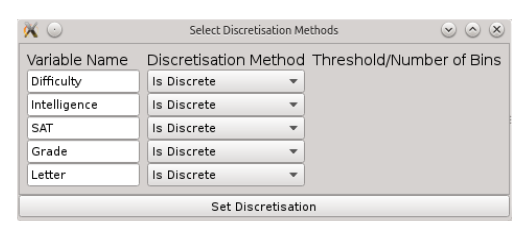
\includegraphics[width=\textwidth]{pic/discretisationInteractive.eps}
  \caption{Discretisation data for the \textit{Student network} can be provided interactively. As the data is discrete in the first place, we chose the \texttt{Is Discrete} option from the Combo Box}.
  \label{figure:chooseDiscInf}
 \end{center}
\end{figure}
\noindent
Once the data and the discretisation information are specified, the model is trained using an expectation maximisation algorithm. The GUI layout changes again, as it can be seen in Figure \ref{figure:guiAfterTraining}.
\begin{figure}[H]
 \begin{center}
  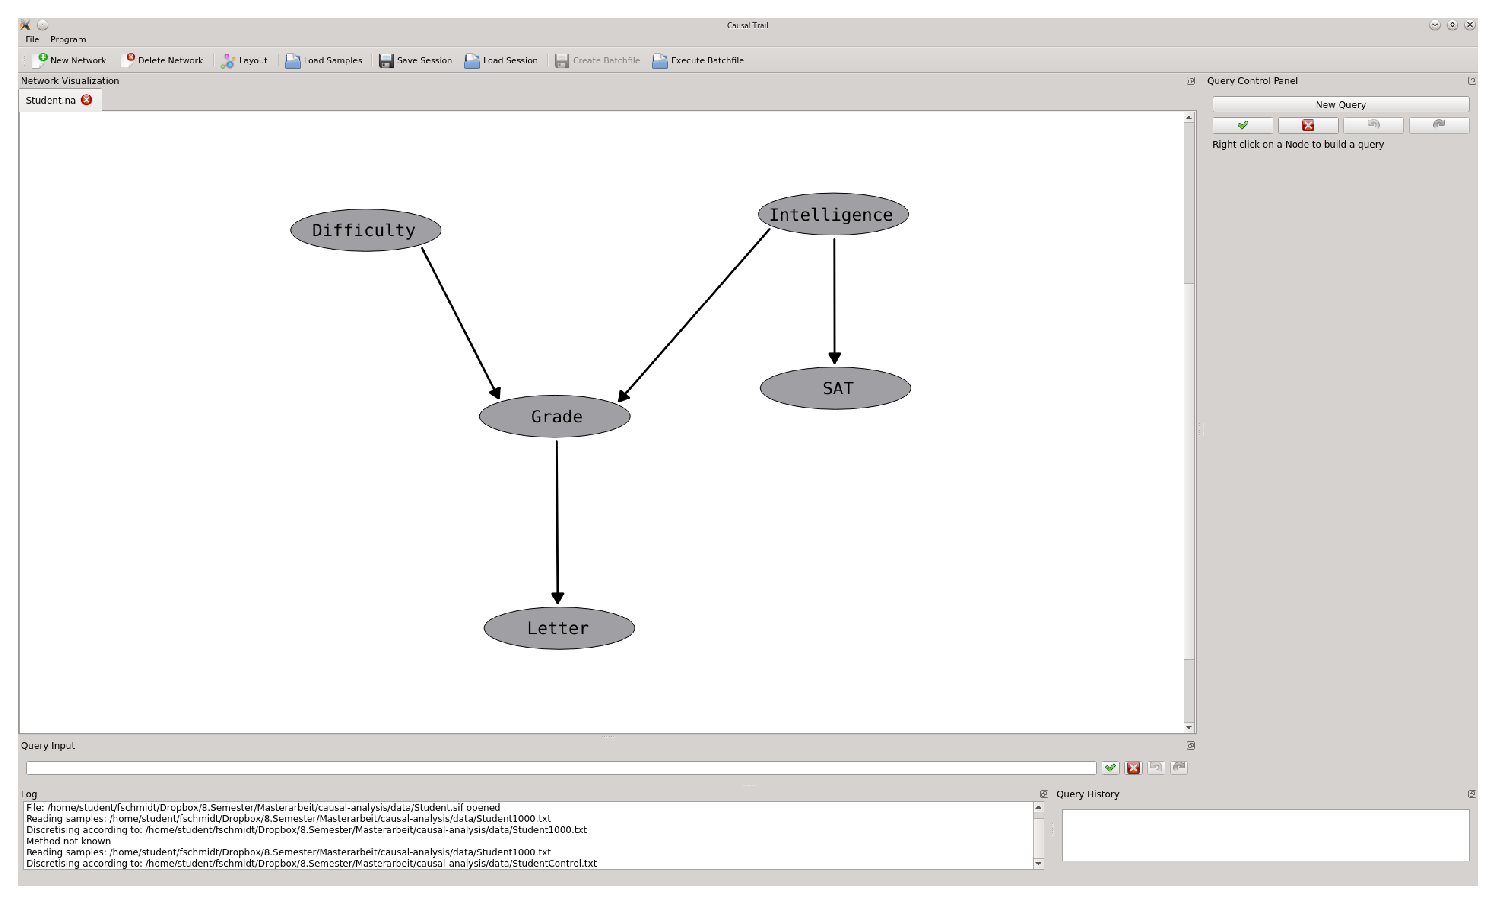
\includegraphics[width=\textwidth]{pic/gui4.eps}
  \caption{Layout of the graphical user interface once the currently represented network is trained.}
  \label{figure:guiAfterTraining}
 \end{center}
\end{figure}
\noindent
There are three new GUI elements. The box \texttt{Query Input} allows the user to enter a query, just like in the console version of \textit{CausalTrail}. Submitted queries are stored in the \texttt{Query History}.
The \texttt{Query Control Panel} allows an interactive query construction. The function of these elements are detailed in Section \ref{subsection:queryFormulation}.

\subsection{Sessions}
\label{subsection:loadSessions}
To simplify the usage of our tool and to avoid repeating the process of network and sample loading, \textit{CausalTrail} supports sessions. A session in \textit{CausalTrail} contains
all currently trained networks, and submitted queries.
To save a session, click on \texttt{Save Session} in the toolbar or click \texttt{File} $\rightarrow$ \texttt{Save Session} in the menu. The dialogue shown in the left part of Figure \ref{figure:Session} appears.
The user has to specify a \textit{CausalTrail Session File (cts)}. To load a stored session, choose \texttt{Load Session} in the toolbar or click \texttt{File} $\rightarrow$ \texttt{Load Session} in the menu. 
The right part of Figure \ref{figure:Session} shows the dialogue to select a \textit{cts} file. Loaded networks will be added to the current session of \textit{CausalTrail}.
\begin{figure}[H]
\begin{minipage}{6cm}
 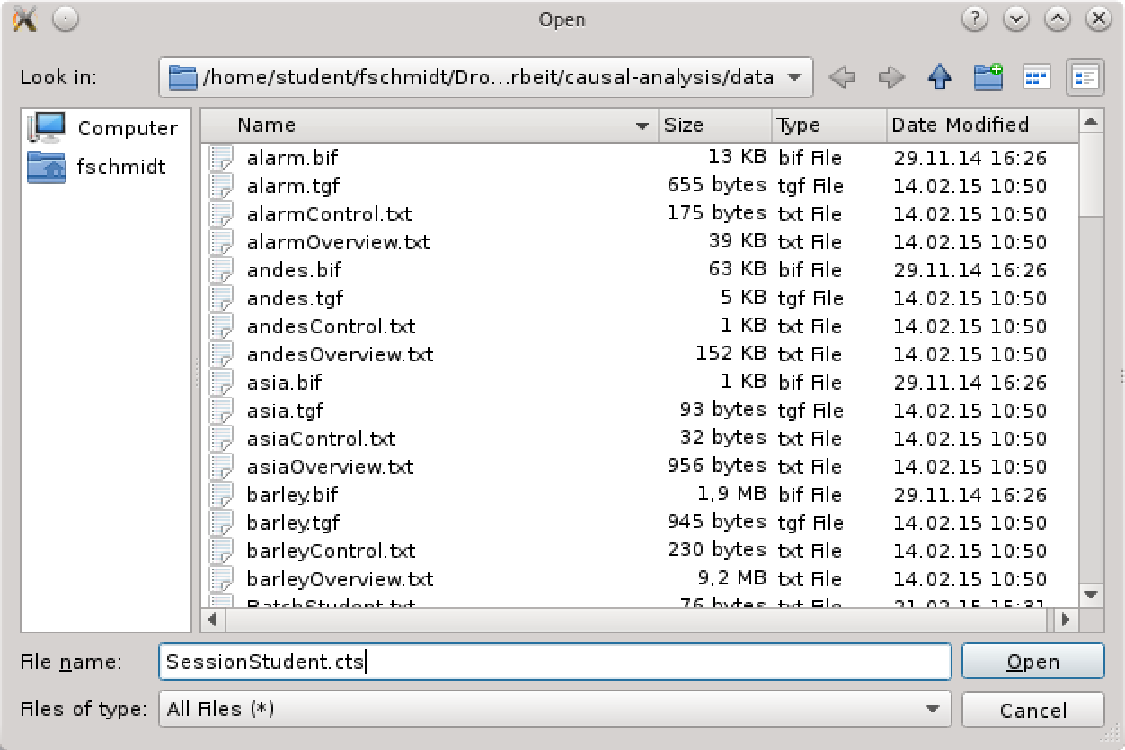
\includegraphics[width=6cm]{pic/saveSession.eps}
\end{minipage}
%
\begin{minipage}{6cm}
 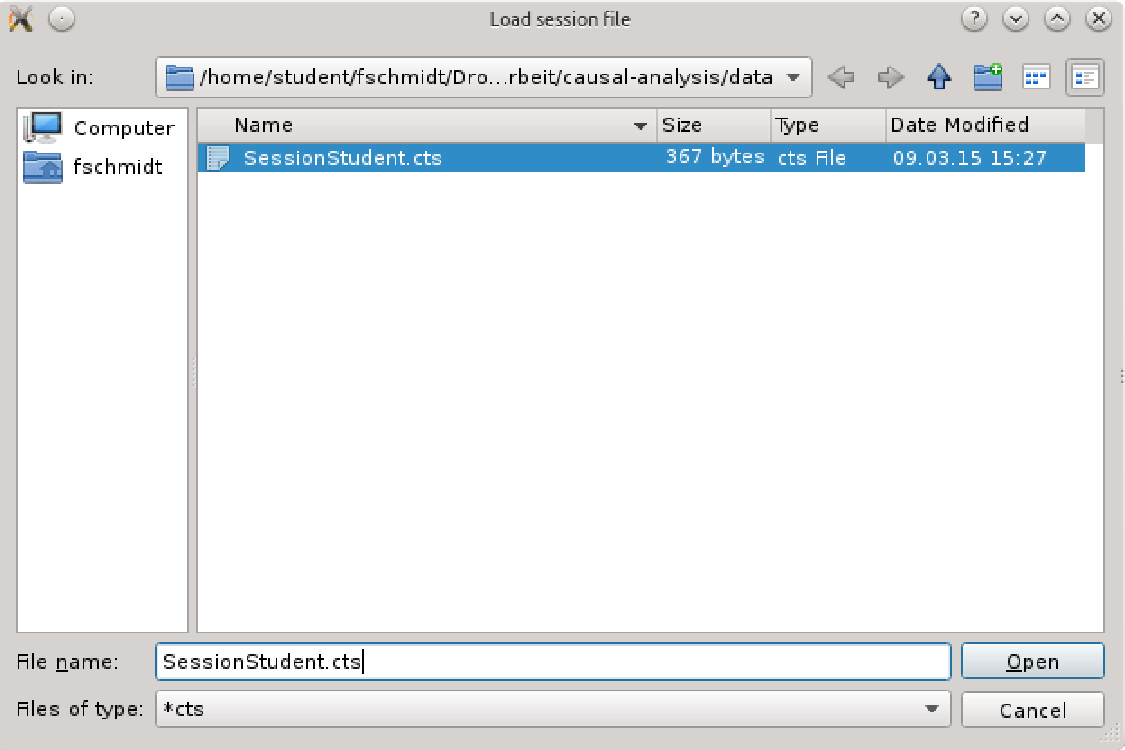
\includegraphics[width=6cm]{pic/loadSession.eps}
\end{minipage}
\caption{Dialogues to handle sessions in \textit{CausalTrail}. The dialogue on the left hand-side can be used to store a session, the dialogue on the right hand-side can be used to load a session. Sessions are stored in
\textit{CausalTrail Session Files (cts)}.}
\label{figure:Session}
\end{figure}

\subsection{View Conditional Probability Tables}
It is possible to view the conditional probability table (CPT) of a node. To view the table, right click on a node. Select \texttt{Show CPT} in the appearing context menu.
A conditional probability table for the selected node pops up. Its name is given in the header of the window. Columns in the CPT with an italic label represent the parent nodes and their respective values. Values of the selected node are written in bold.
Figure \ref{figure:CPTs} shows an example for a CPT of node \textit{Grade} in the \textit{Student network}.
\begin{figure}[H]
  \begin{minipage}{6cm}
  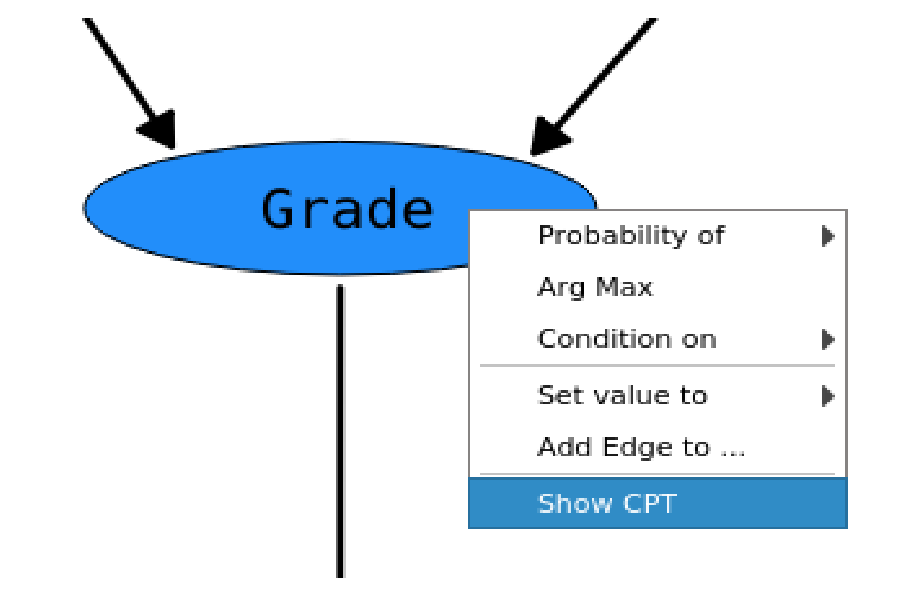
\includegraphics[width=6cm]{pic/loadCPT.eps}
  \end{minipage}
  %
  \begin{minipage}{6cm}
 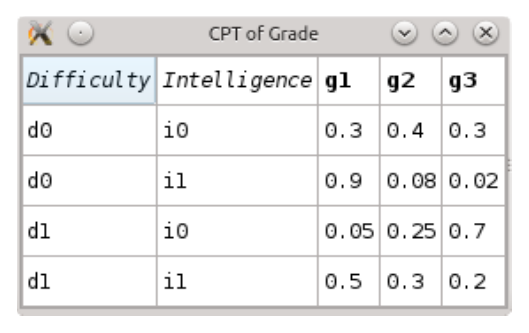
\includegraphics[width=6cm]{pic/cpt.eps}
  \end{minipage}
  \caption{The left part of this figure shows how to open a conditional probability table. The table itself is depicted in the right part of the figure. The name of the represented node is given in the header of the window. Columns in the CPT with an italic label
  represent the parent nodes and their respective values.}
  \label{figure:CPTs}
\end{figure}


\subsection{Queries}
\label{subsection:queryFormulation}
\textit{CausalTrail} offers three ways to submit a query. A query can be
\begin{enumerate}
  \item entered directly, as in the console version of \textit{CausalTrail}.
  \item entered interactively, by clicking on the nodes of the network and selecting their desired state.
  \item chosen from the \texttt{Query History}, containing all previously submitted queries of the current session.
\end{enumerate}
The following sections cover these options in detail.  
\bigskip
\\The result of query is shown in the \texttt{Log} and in the \texttt{Query Control Panel}. Submitted queries are listed in the 
\texttt{Query History}.

\subsubsection{Direct Query Formulation}
Queries can be entered directly using the \texttt{Query Input} widget. A query can be submitted by pressing \textit{Enter} or by a click on the green tick.
An example is shown in Figure \ref{figure:queryDirect}.
\begin{figure}[H]
 \begin{center}
  
\includegraphics[width=6cm]{pic/queryInputDirect.eps}
  \caption{Direct input of queries using the \texttt{Query Input} widget. Queries are submitted by a click on the green tick, or by pressing \textit{Enter}. Clicking on the red cross resets the result box in the \texttt{Query Control Panel}.}
  \label{figure:queryDirect}
 \end{center}
\end{figure}
\noindent
Entering queries directly requires the user to be familiar with our query language. As this can not be expected from the general user, \textit{CausalTrail}
allows an interactive query construction, introduced in the next section.

\subsubsection{Interactive Query Construction}
Queries can be built interactively by the user. This permits the user to formulate queries without learning our query language.
To start building a query, the user has to move the mouse over a node that should be a part of the query.
A right click opens a context menu, as shown in Figure \ref{figure:menu}.
\begin{figure}[H]
  \begin{minipage}{6cm}
  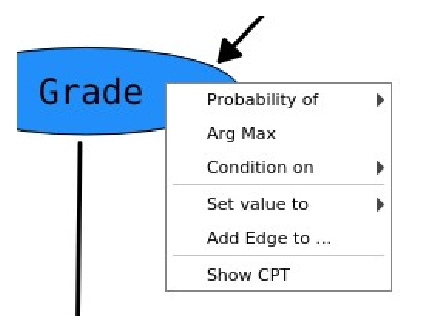
\includegraphics[width=6cm]{pic/menu1.eps}
  \end{minipage}
  %
  \begin{minipage}{6cm}
 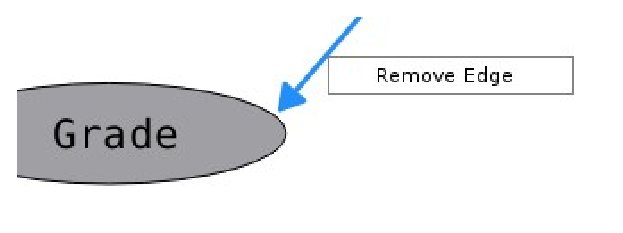
\includegraphics[width=4cm]{pic/menu2.eps}
  \end{minipage}
  \caption{The left hand-side shows the context menu for nodes, the right hand-side shows the context menu for edges. The context menus are empty if the network is not trained.}
  \label{figure:menu}
\end{figure}
There are five options related to query construction:
\begin{enumerate}
 \item Probability of: Calculates the probability that this node obtains the specified value.
 \item Arg Max: Calculates the most likely value assignment for this node. It is not possible to combine (1) and (2).
 \item Condition on: Conditioning the probability of other nodes on the specified value of the currently selected one.
 \item Set Value to: Performs a do-intervention on the current node. The edges to its parents are deleted, and its own value is fixed to the selected one.
 \item Add Edge to: Adds an edge to another node. To add a new edge double click on the desired target node. The added edge will appear in red. If the new edge would induce a cycle, an error will be shown in the \texttt{Log}.
 Adding an edge triggers retraining of the entire network.
\end{enumerate}
Once an item is selected, it appears in the \texttt{Query Control Panel}. Double clicking on an item in one the boxes in the \texttt{Query Control Panel} removes them from the current query.
A colour code simplifies the identification of different query elements. A natural language wrapper around the query element boxes further facilitates the understanding of the query.
\bigskip
\\In addition to the operations on nodes, there is an operation on edges. A right click on an edge opens a context menu, as shown in Figure \ref{figure:menu}. Selecting \texttt{Remove Edge} removes the selected edge.
Removed edges, are shown in grey. The style of the edge is changed from solid to dashed. As for adding an edge, removing one also triggers retraining of the network.
An example containing all types of actions, except the \textit{Arg Max} setting is shown in Figure \ref{figure:exampleInteractive}.
\begin{figure}[H]
 \begin{center}
  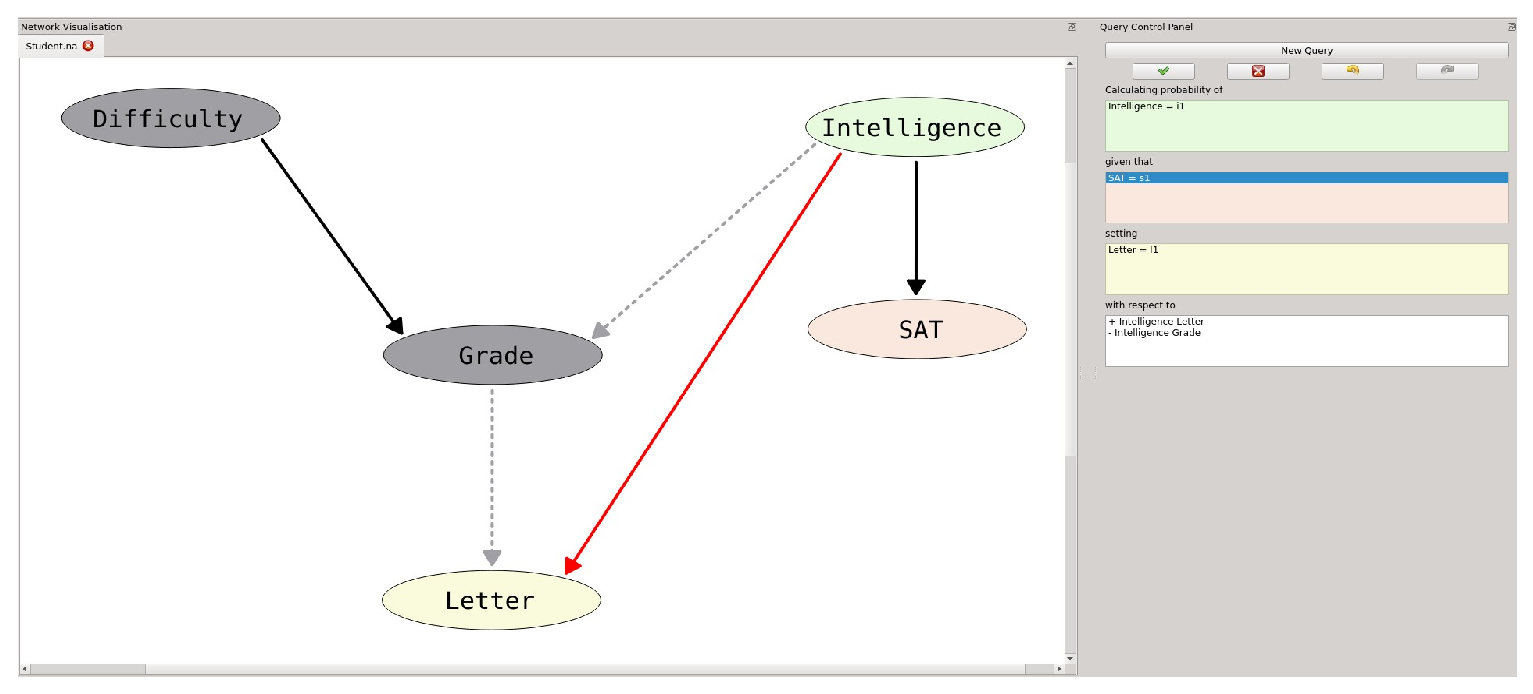
\includegraphics[width=\textwidth]{pic/exampleAll.eps}
  \caption{An example query in the \textit{Student network}. In this example, we compute the probability that
  Intelligence has the value i1, given the SAT has the value s1, Letter is set to l1, there is an additional edge
  from Intelligence to Letter, and the edge from Intelligence to Grade is removed. 
  Conditions are shown in bright red, do interventions in yellow, query probabilities in green.
  Additional edges are red, removed edges are dashed and shown in grey.}
  \label{figure:exampleInteractive}
 \end{center}
\end{figure}
\noindent
A query can be calculated either by clicking on the green tick in the \texttt{Query Control Panel}, or by pressing \textit{Enter}.
To enter a new query, the button \texttt{New Query} has to be clicked.

\subsubsection{Query History}
Queries are stored in the \texttt{Query History}. There are two ways to reload a query contained in the history.
\begin{enumerate}
 \item A query can be directly selected via a double click in the \texttt{Query History} box, as shown in Figure \ref{figure:history}. 
 \item Using the yellow and green arrows in the \texttt{Query Input} and in the \texttt{Query Control Panel}, the user can shift through all previously submitted queries
\end{enumerate}
The visualisation of the network and the \texttt{Query Control Panel} are adapted according to the selected query.
\begin{figure}[H]
 \begin{center}
  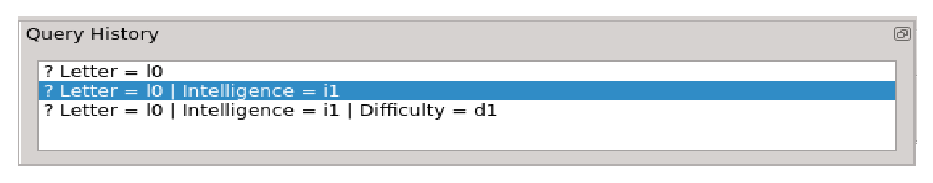
\includegraphics[width=\textwidth]{pic/queryHistory.eps}
  \caption{The \texttt{Query History} widget lists all valid, submitted queries. Double clicking a query reloads it. The network visualisation and the \texttt{Query Control Panel} are updated according to the query. In this example, the second query is selected.}
  \label{figure:history}
 \end{center}
\end{figure}

\subsection{Query Batch Files}
To allow the user to quickly process a set of queries with networks trained on different data, \textit{CausalTrail} offers \textit{Query Batch Files}. 
A batch file can be created by clicking on \texttt{Create Batchfile}. Queries currently shown in the \texttt{Query History} are written to the batchfile.
A batchfile can be executed by a click on \texttt{Execute Batchfile}. Results are shown in the \texttt{Log}.

\subsection{Example Queries}
To illustrate the usage of \textit{CausalTrail} further, we present a few example Queries in the \textit{Student Network}.
\subsubsection{Predictions}
In Figure \ref{figure:p1} we show a query to compute the probability of Intelligence obtaining the value i1. Figure \ref{figure:p2} shows a query including a condition.
There, we compute the probability that Intelligence obtains the value i1, if Grade has the value g1 and SAT has the value s1.
\begin{figure}[H]
 \begin{center}
  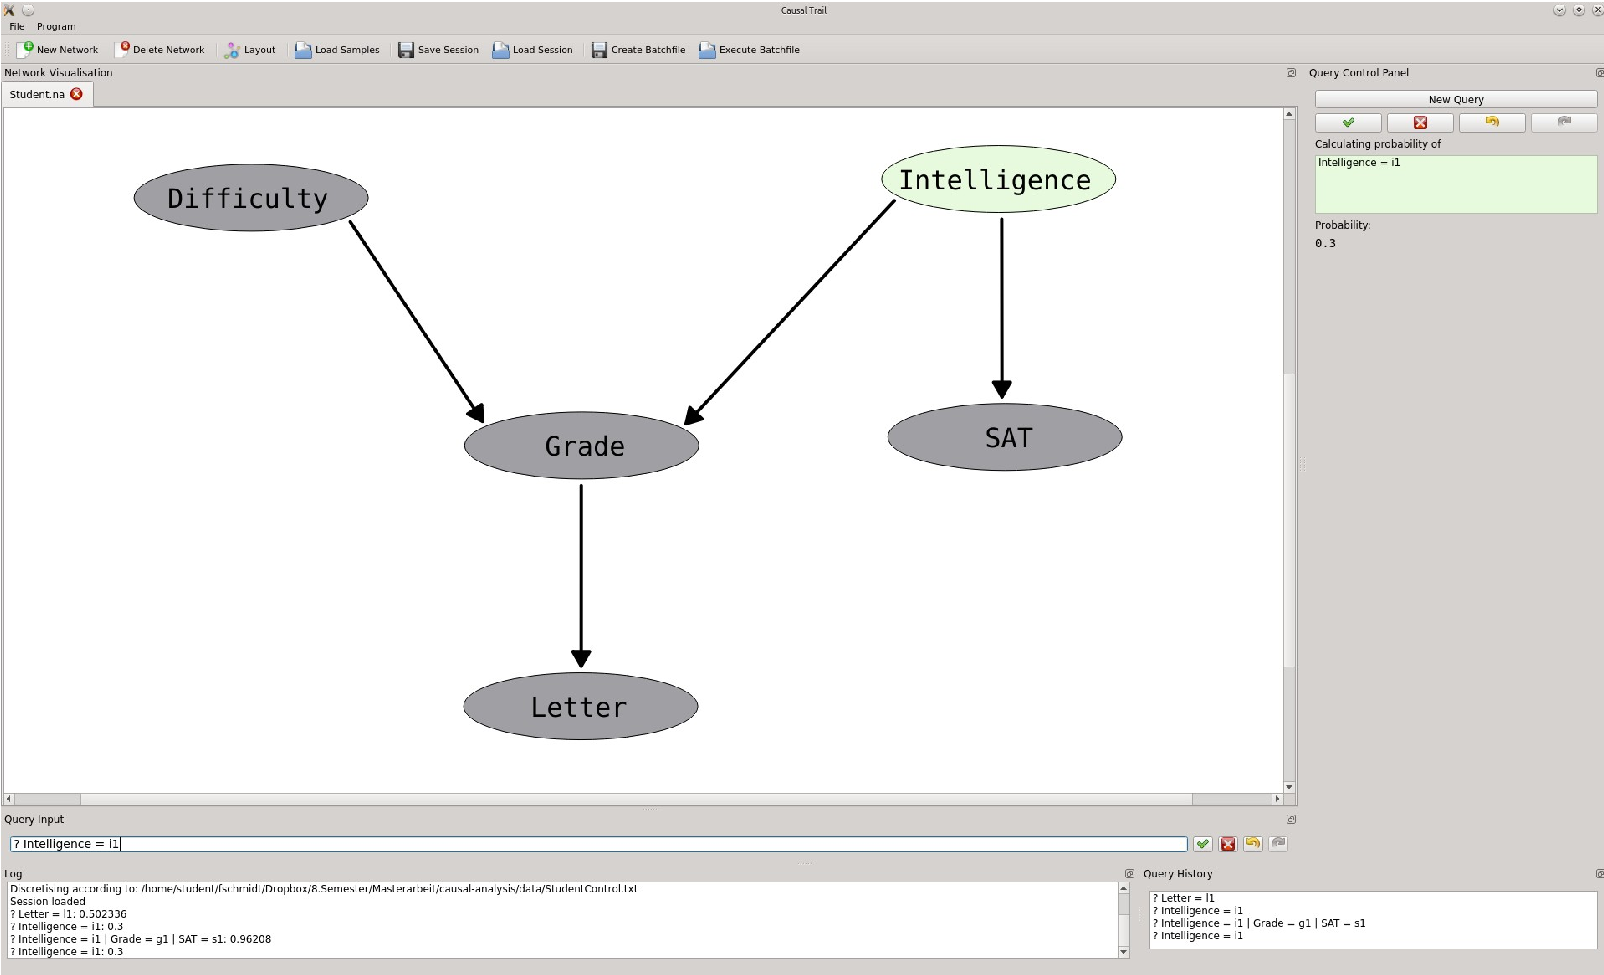
\includegraphics[width=\textwidth]{pic/p1.eps}
  \caption{Example for a simple prediction: Computing the query \texttt{? Intelligence = i1}.}
  \label{figure:p1}
 \end{center}
\end{figure}
\begin{figure}[H]
 \begin{center}
  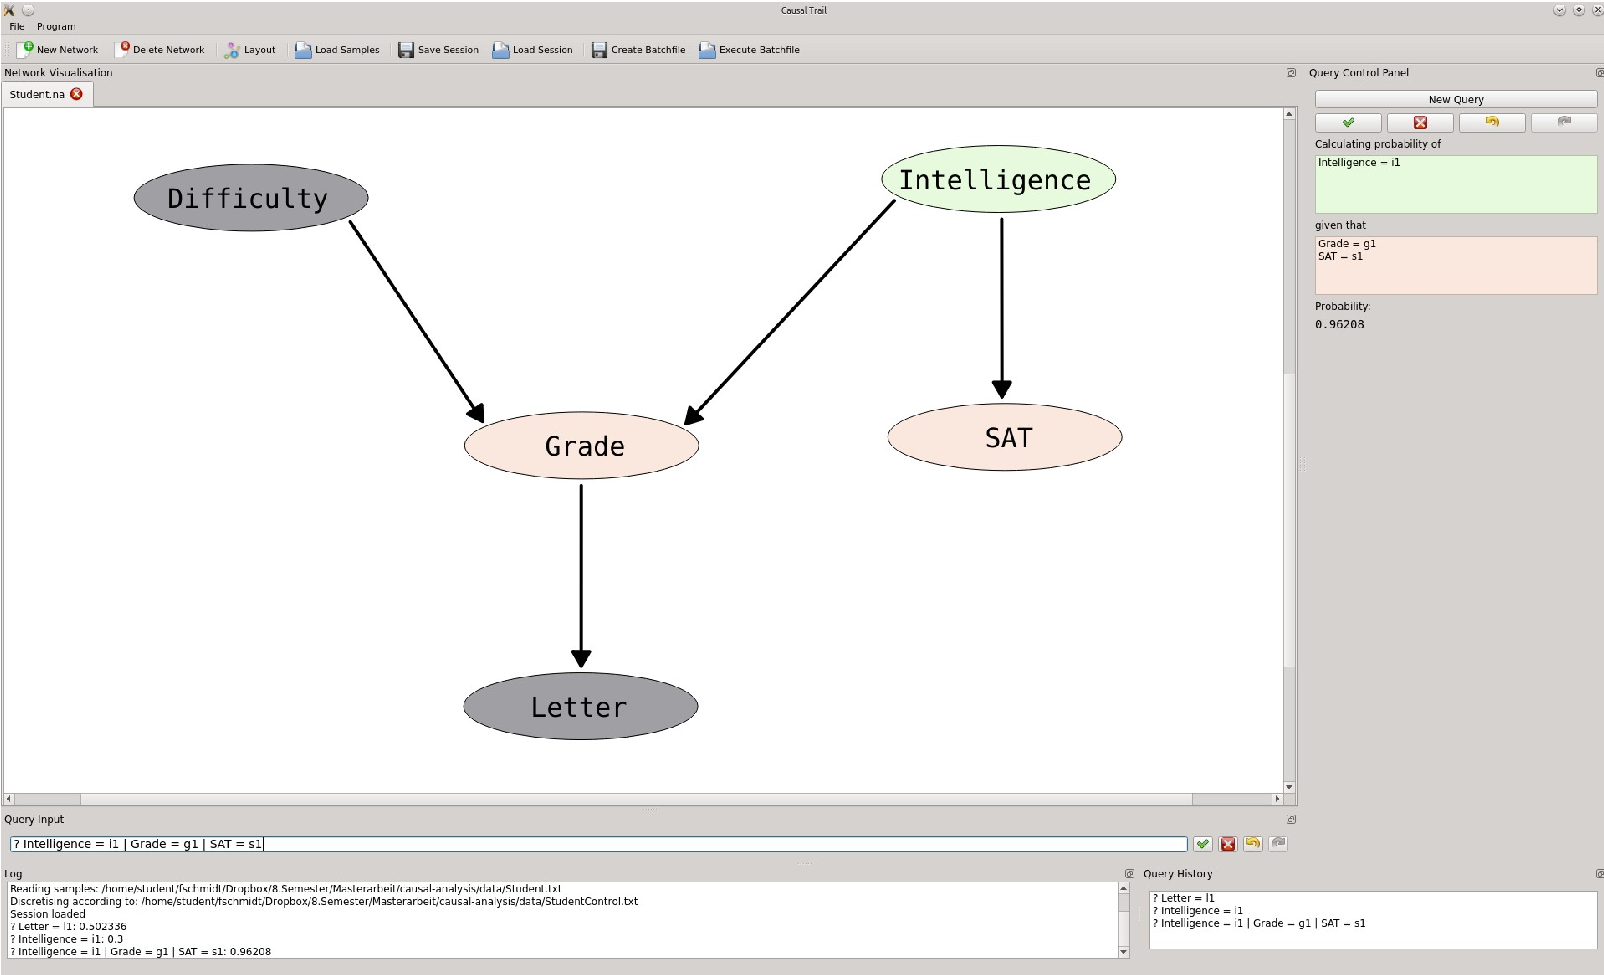
\includegraphics[width=\textwidth]{pic/p2.eps}
  \caption{Example for prediction together with a condition: Computing the query \texttt{? Intelligence = i1 | Grade = g1 SAT = s1}.}
  \label{figure:p2}
 \end{center}
\end{figure}

\subsubsection{Interventions}
The query shown in Figure \ref{figure:i1} contains a do-intervention. We compute the probability of Intelligence obtaining the value i1, given that SAT has the value s1 and we set the value of Grade to g1.
\begin{figure}[H]
 \begin{center}
  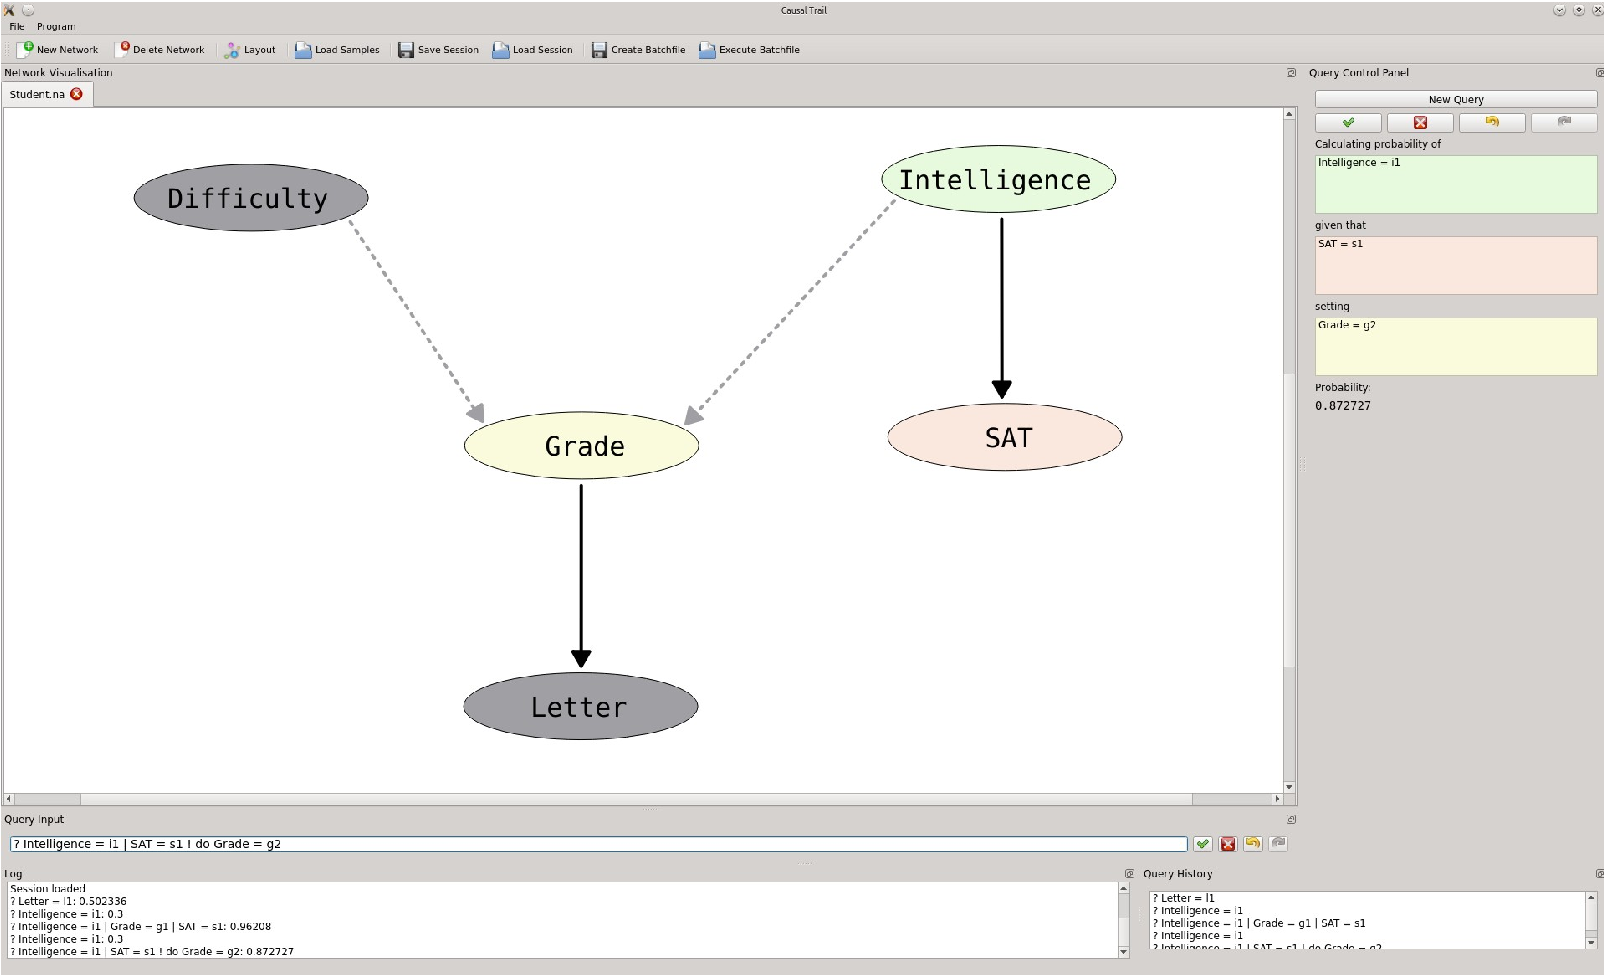
\includegraphics[width=\textwidth]{pic/i1.eps}
  \caption{Example for a do intervention: Computing the query \texttt{? Intelligence = i1 ! do Grade = g1 | SAT = s1}.}
  \label{figure:i1}
 \end{center}
\end{figure}

\subsubsection{Counterfactuals}
Figure \ref{figure:c} represents a counterfactual. We compute the probability to get a letter, if we  have not received a letter before.
\begin{figure}[H]
 \begin{center}
  \includegraphics[width=\textwidth]{pic/c1.eps}
  \caption{Example for a counterfactual: Computing the query \texttt{? Letter = l1 | Letter = l0}.}
  \label{figure:c}
 \end{center}
\end{figure}
